\documentclass{standalone}
\usepackage{tikz}
\usetikzlibrary{decorations.pathreplacing, patterns, decorations.pathmorphing, decorations.text}

\begin{document}
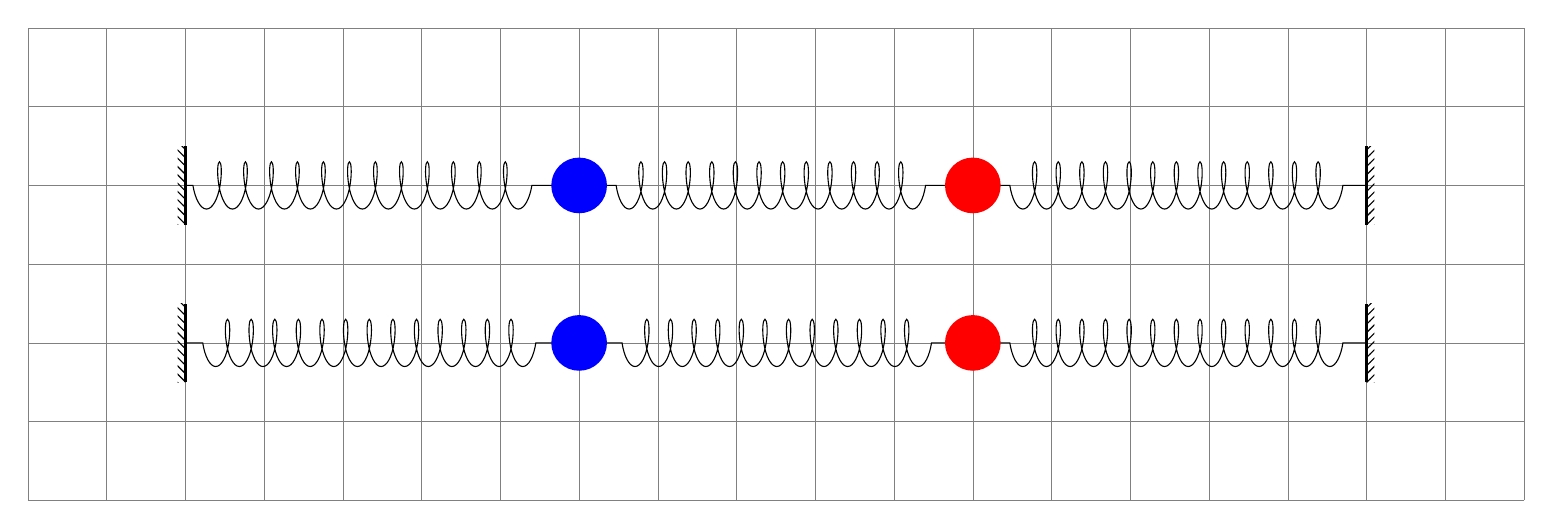
\begin{tikzpicture}

%grid help
 \draw[gray, very thin] (-12,-4) grid (7,2);

% Define coordinates
\coordinate (leftSupport) at (-10,0);
\coordinate (rightSupport) at (5,0);
\coordinate (massA) at (0,0);
\coordinate (massB) at (-5,0);
\coordinate (springEndA) at (5,0);
\coordinate (springEndB) at (-10,0);

% Left supporting structure
\fill [pattern=north west lines] (leftSupport) ++(-0.1,-0.5) rectangle ++(0.1,1);
\draw[thick] (leftSupport) ++(0,-0.5) -- ++(0,1);

% Right supporting structure
\fill [pattern=north east lines] (rightSupport) ++(0,-0.5) rectangle ++(0.1,1);
\draw[thick] (rightSupport) ++(0,-0.5) -- ++(0,1);

% Spring between mass A and right support
\draw[decorate, decoration={aspect=0.3, segment length=3mm, amplitude=3mm, coil, pre length=3mm, post length=3mm}] 
    (springEndA) -- (massA);

% Spring between mass A and mass B
\draw[decorate, decoration={aspect=0.3, segment length=3mm, amplitude=3mm, coil, pre length=6mm, post length=3mm}] 
    (massA) -- (massB); 

% Spring between mass B and left support with fewer loops
\draw[decorate, decoration={aspect=0.3, segment length=3.3mm, amplitude=3mm, coil, pre length=6mm, post length=0.75mm}] 
    (massB) -- (springEndB);

% Mass A
\node[circle, fill=red, inner sep=2.5mm] (a) at (massA) {};

% Mass B
\node[circle, fill=blue, inner sep=2.5mm] (b) at (massB) {};



%%%%%%%%%%%%%% Second Pattern starts here %%%%%%%%%%%%%%%%%%%%%%%%%%

\coordinate (leftSupport) at (-10.0,-2.0);
\coordinate (rightSupport) at (5.0,0);
\coordinate (massA) at (0.0,-2);
\coordinate (massB) at (-5.0,-2);
\coordinate (springEndA) at (5.0,0);
\coordinate (springEndB) at (-5.0,0);




% Left supporting structure
\fill [pattern=north west lines] (leftSupport) ++(-0.1,-0.5) rectangle ++(0.1,1);
\draw[thick] (leftSupport) ++(0,-0.5) -- ++(0,1);

% Right supporting structure
\fill [pattern=north east lines] (rightSupport) ++(0,-0.5)++(0,-2) rectangle ++(0.1,1)++(0,-2);
\draw[thick] (rightSupport) ++(0,-0.5)++(0,-2) -- ++(0,1)++(0,-2);

% Spring between mass A and right support
\draw[decorate, decoration={aspect=0.3, segment length=3mm, amplitude=3mm, coil, pre length=3mm, post length=3mm}] (springEndA)++(0,-2) -- (massA)++(-2.5mm,0);


% Spring between mass A and mass B
\draw[decorate, decoration={aspect=0.3, segment length=3mm, amplitude=3mm, coil, pre length=3mm, post length=3mm}] (massA)++(-2.25mm,0) -- (massB) -- ++(0.5mm,0); 
%% Fix suggested by Joe Heafner inserted above.


% Spring between mass B and left support
\draw[decorate, decoration={aspect=0.3, segment length=3mm, amplitude=3mm, coil, pre length=3mm, post length=0mm}] (springEndB)++(-2.5mm,0)++(0,-2) -- (leftSupport)++(0,-2);

% Mass A
\node[circle, fill=red, inner sep=2.5mm, anchor=center] (a) at (massA) {};

% Mass B
\node[circle, fill=blue, inner sep=2.5mm, anchor=center] (b) at (massB) {};


% Connecting lines to support structures
%\draw[] (springEndA) -- (rightSupport);
%\draw[] (springEndB) -- (massB);

\end{tikzpicture}
\end{document}
